\documentclass[letter,12pt]{article}


\usepackage[english]{babel}

\usepackage{fancyhdr}


\usepackage{graphicx}
\usepackage{amsmath}
\usepackage{amssymb}
\usepackage[latin1]{inputenc}
\usepackage{fancybox}
\usepackage{amsfonts}
\usepackage{bbold}
\usepackage{textcomp}


\setlength{\oddsidemargin}{0in}
\setlength{\evensidemargin}{0in}
\setlength{\textwidth}{16.1 cm}
\setlength{\topmargin}{-15mm}
\setlength{\textheight}{22cm}
\setlength{\parindent}{0cm}


\newcommand{\sv}{\underline}
\newcommand{\Sig}{\boldsymbol{\sigma}}
\newcommand{\K}{\boldsymbol{K}}
\newcommand{\Eps}{\boldsymbol{\varepsilon}}
\newcommand{\intener}{\mathcal{E}}


% --------------------------------------------------------------------------------------
% - definition des notations
% --------------------------------------------------------------------------------------


% - tenseur d'ordre 4
\newcommand{\TTTT}[1]{\underline{\underline{\underline{\underline{#1}}}}}
% - tenseur d'ordre 2
\newcommand{\TT}[1]{\underline{\underline{#1}}}
% - tenseur d'ordre 1
\newcommand{\T}[1]{\underline{#1}}

% - composante i - j de la contrainte: 
\newcommand{\sigi}[1]{\sigma_{#1}}
% - composante i - j de la deformation: 
\newcommand{\epsi}[1]{\varepsilon_{#1}}

% - tenseur de contrainte : 
\newcommand{\sig}{\TT{\sigma}}
\newcommand{\eps}{\TT{\varepsilon}}
\newcommand{\C}{\TTTT{C}}
\renewcommand{\S}{\TTTT{S}}

% - composantes des tenseurs de Hooke: 
\newcommand{\Ci}[1]{C_{#1}}
\newcommand{\Si}[1]{S_{#1}}

% - notations pour un vecteur
\renewcommand{\Vec}[1]{\underline{#1}}


% - notations pour un vecteur chapeau
\newcommand{\Vecc}[1]{\hat{\underline{#1}}}

% - notations pour un produit tensoriel
\newcommand{\tens}[2]{#1 \otimes #2}

% - notations pour les vecteurs de base
\newcommand{\e}[1]{\Vec{e_{#1}}}

% - contrainte equivalente pour les crit�res de plasticite
\newcommand{\se}{\sigma_{eq}}

% - deformation elastique
\newcommand{\epse}{\TT{\varepsilon_e}}

% - deformation elastique
\newcommand{\epsp}{\TT{\varepsilon_p}}


\begin{document}
\pagestyle{fancy}

\title{\textbf{Static admissibility \#3}}
\date{}

\maketitle



We consider a closed tube associated with a cylindrical coordinate system $(\underline{O}, \underline{e}_r, \underline{e}_{\theta}, \underline{e}_z)$. \\

The tube is subjected to an internal pressure $p_i$. All other surfaces are free of stresses.


\begin{description}
\item \textbf{Question:} Write all the equations defining static admissibility  for $\TT{\sigma}$ (no expansion needed at this time).
\item \textbf{Question:} Expand these equations. 
\end{description}


%
%------------------------------------------------------------------------
\begin{figure}[!h]
	\centering
	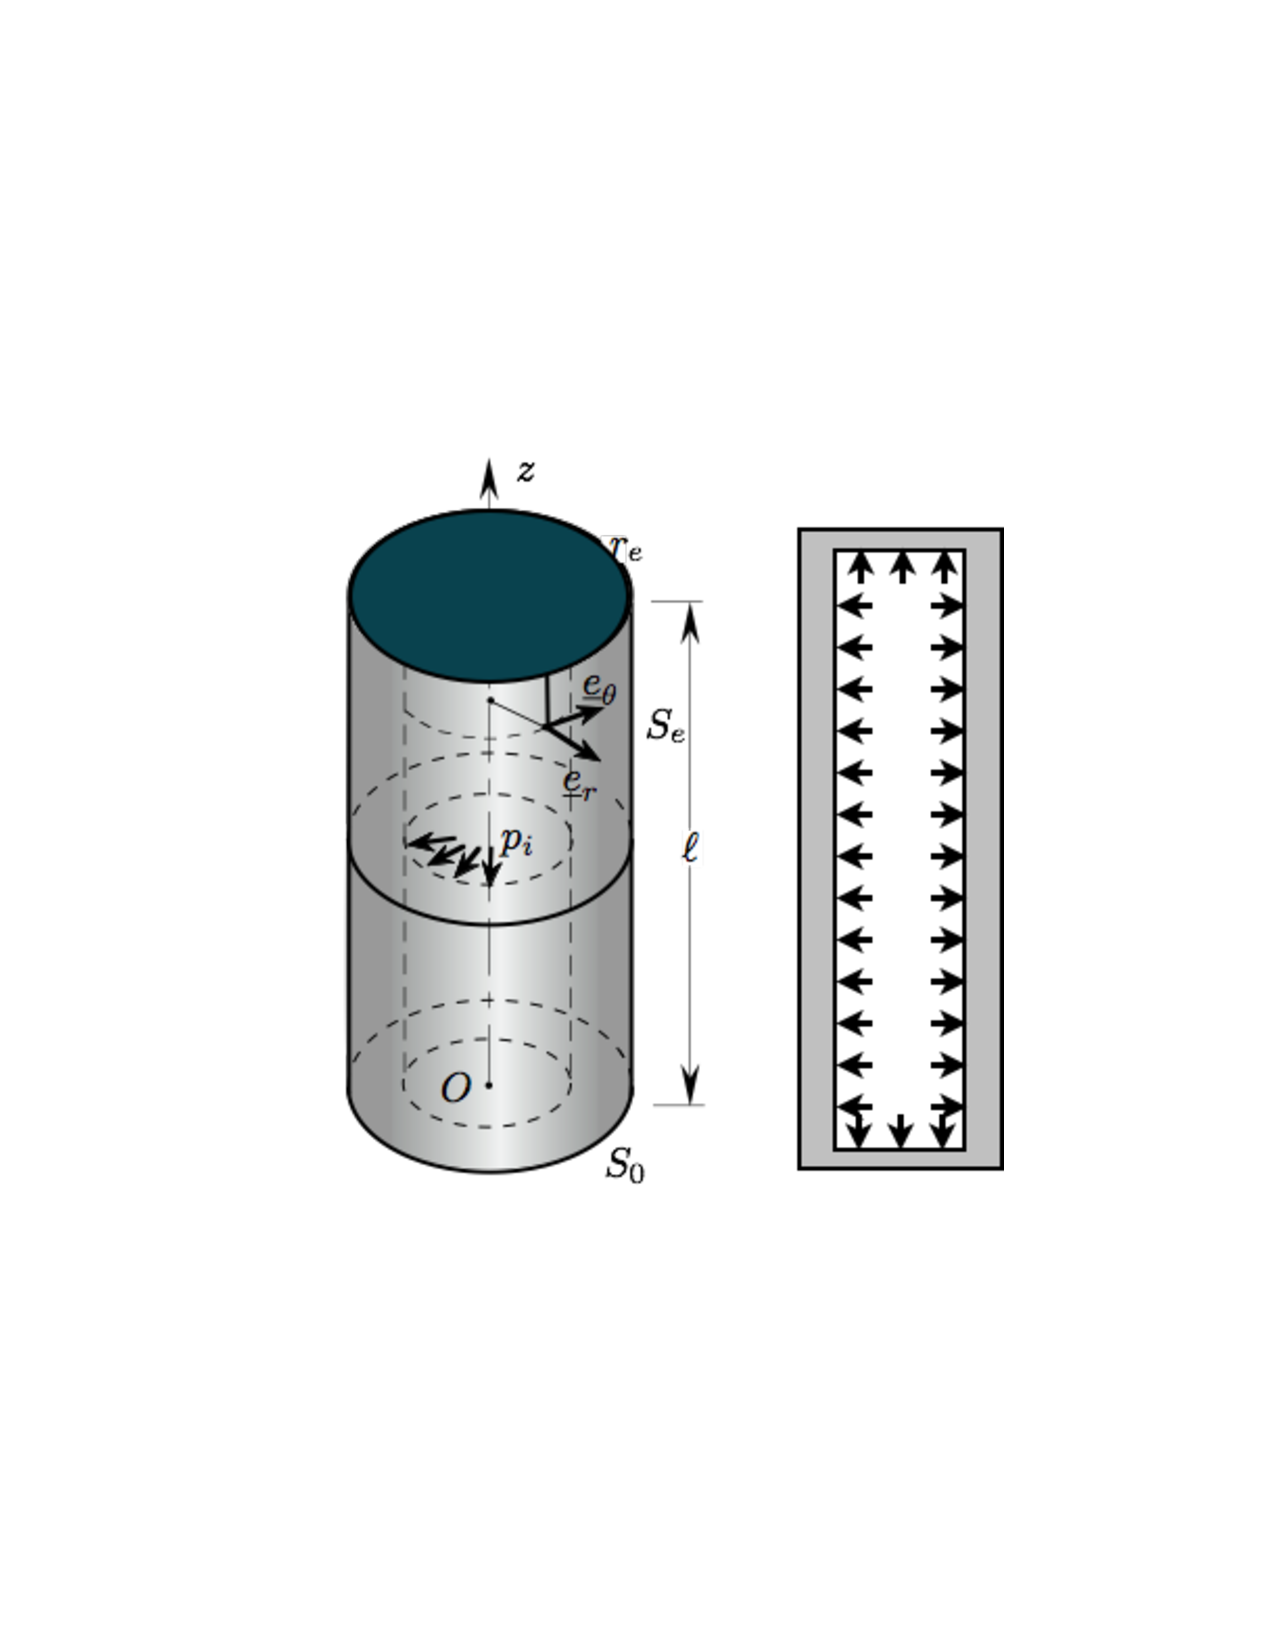
\includegraphics[width=0.5\linewidth]{./volume}
	\caption{}
\end{figure}
%------------------------------------------------------------------------
%









\end{document}